\chapter{Majorana Fermions \label{chap:Majorana}}

The  Majorana Fermions, so called in the name of the Italian physicist Ettore Majorana, were first defined in the attempt to find a real solution of the Dirac equation. The real field that solves this equation describes a fermion which is its own antiparticle. Hence it has no electric charge  nor mass.  Till these days, no fundamental particle with these characteristics has been observed. However, in the last decade, there has been a huge speculation about the possibility of finding Majorana Fermions as a quasi-particles of certain types of topological superconductors.

The topological materials are a novel type of material that experiences phase transitions without any symmetry breaking. As consequence, they cannot be characterized by the Landau theory. Instead, the phase transition is characterized with a topological order . Since topological characters are discrete parameters that describe non-local features of the material, the phases with this characterization present robust characteristics that are difficult to alter. An example of this is the quantum hall effect which robustness is famous and widely used in high precision devices. 

One of the most promising topological materials is the one dimensional majorana wire. This wire is inspired in a famous Kitaev's toy model representing a spinless p-wave superconducting wire. Under certain conditions, the majorana wires experience topological phase transition characterized by the emergence exotic zero-modes localized at edges of the wire. Kitaev associated these modes with majorana quasi-particles  appearing at the boundary of the topological superconducting wire. Moreover, he pointed out that the combined used of robustness from topological materials and Majorana's non-abelian statistics could lead to the creation of fault tolerant quantum gates. This fact opened the doors to the search of majorana fermions in condensed matter physics. 

In this chapter we will present a review of the main topics about majorana fermions. In the first section \ref{sec:KitaevChain}, we will describe the the Kitaev's chain and the emergence of majorana zero modes. Next, we will discuss about the real implementations of majorana chains and the experimental proposals that have been carried on . Finally, we will take a look to the results coupling QDs with majorana chains.


% ------------------------Section: Kitaev *------------------
\section{The Kitaev Chain \label{sec:KitaevChain}}
In this section we discuss the main aspects of Kitaev's toy model. This is a toy model in tight binding that represents a  finite $p$-wave superconducting wire with the following Hamiltonian

\begin{equation}
H = \sum_{i} \left[ -t(a_i^{\dagger} a_{i+1} + a_{i+1}^{\dagger}a_i) -\mu a_i^{\dagger} a_{i} +  \Delta a_{i}a_{i+1} + \Delta^* a_{i+1}^{\dagger}a_i^{\dagger} \right].  \label{eq:kitaevHam}
\end{equation}

Where $\mu$ is the chemical potential, so that $\mu a_i^{\dagger} a_{i}$ is the energy associated to each step in the chain. $t(a_i^{\dagger} a_{i+1} + a_{i+1}^{\dagger}a_i)$ represents the interaction between neighbouring sites which is determined by the hopping term $t$. The remaining terms describe the superconducting properties of the system as is is established by the BCS theory of superconductivity. $\Delta$ is a complex superconducting parameter with the form  $\Delta = e^{i\theta} \super$. The associated terms represent the Cooper pairs which can be created or annihilated at neighbouring sites of the system.

The form of hamiltonian \prettyref{eq:kitaevHam} favors the possibility of introducing new operators $\gammaA{j}$ and $\gammaB{j}$ such that

\begin{equation}
\gammaA{j} = e^{i\theta /2}a_j+ e^{-i\theta/2 } \ann_j \ \ , \ \ \gammaB{j} = -i(e^{i\theta /2}a_j - e^{-i\theta/2} \ann_j).
\label{eq:majoranaTrans}
\end{equation}
It is simple check that these operators are self-adjoint $(\gammaA{j}^\dagger = \gammaA{j}, \gammaA{j}^\dagger = \gammaB{j})$. This is a required constraint for the Majorana particles. In addition they satisfy the fermionic anti-commutation relations
\begin{equation}
\begin{aligned}
\{\gammaA{i}, \gammaA{j}\} = \{ & \gammaB{i} , \gammaB{j}\} = 2\delta_{ij}  ,\\ 
  \{\gammaA{i}, \gammaB{j} & \} =0.
\end{aligned} 
\label{majoranaRel}
\end{equation} 
This allows us to understand the operators $\gammaA{i} , \gammaB{i}$ as majorana fermions. If we also take the inverse of \prettyref{eq:majoranaTrans} we obtain that each  (Dirac) fermion in Hamiltonian \eqref{eq:kitaevHam} is composed by two majorana fermions such that 
$$a_j = \frac{e^{-i\theta/2}}{2}(\gammaA{j}+ i\gammaB{j})$$
We could even adventure to say that these majorana operators are actually dividing the Dirac fermions into real($\gammaA{}$) and imaginary $(\gammaB{})$ part ,the same way as complex numbers are a composite of two real numbers. 

The new Kitaev Hamiltonian in the Majorana representation looks like 

\begin{equation}
H = \frac{i}{2} \sum_{j} \left[ -\mu \gammaA{j}\gammaB{j}  + (t- \super) \gammaB{j}\gammaA{j+1} + (t+ \super) \gammaA{j}\gammaB{j+1} \right]+Const,\label{eq:HamMajorana}
\end{equation}

Depending on the values of parameters $\mu, t$ and $\super$ we can identify two regimes represented by the following situations:


%\begin{figure}[t]
%$$\includegraphics[scale=0.5]{KitaevtopPhases.jpg}
%\centering
%\label{top.phases kitaev}
%\caption{{\small \textit{Taken from \cite{bernevig2015topological}. Ilustration of the Kitaev chain for open boundary conditions in the Majorana representation. a)Represents the trivial case where the hopping and the superconducting term approaches to $0$. b) The non-trivial topological phase. The coupling is produced between Majoranas in different Dirac fermions }}}
%\end{figure}

\begin{figure}[hbt]
    \centering
    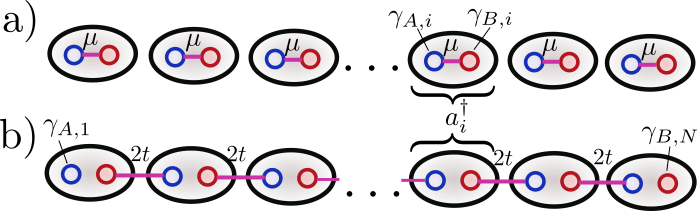
\includegraphics[scale=0.5]{IMAGES/Majorana/KitaevChain.png}
    \label{fig:top.phases kitaev}
    \caption{Illustration of the Kitaev chain for open boundary conditions in the Majorana representation. a)Represents the trivial case where the hopping and the superconducting term approaches to $0$. b) The non-trivial topological phase. The coupling is produced between Majoranas in different Dirac fermions \protect\Source{By the author} }
\end{figure}


\begin{enumerate}
\item{If $\super = t = 0, \mu <0$} Hamiltonian \eqref{eq:HamMajorana} becomes $\frac{-i\mu}{2} \sum_{j} \gammaA{j}\gammaB{j}$ which represents the coupling of the Majoranas in the same Dirac fermion. (See Figure \ref{fig:top.phases kitaev} (a))

\item{If $\super = t > 0, \mu =0$} the situation is much more interesting. The Hamiltonian \eqref{eq:HamMajorana} takes the form $H = 2ti\sum_{j} \gammaA{j}\gammaB{j+1}$. This implies that the coupling is performed between  Majoranas of different Dirac fermions leaving the edge Majorana operators ($\gammaA{1}$ and $\gammaB{N}$) uncoupled (See Figure \ref{fig:top.phases kitaev}b)). Note that these uncoupled majorana fermions can be at any state without any  repercussion in the energy of the system. This explains the emergence of a  ground state localized at edges of the chain. 
\end{enumerate}

These two situations are representatives of two different phases that can be characterized by a topological parameter. To understand this characterization we need to take a look to the spectrum of Hamiltonian \ref{eq:Majorana-ham}.

\begin{figure}[hbt]
    \centering
    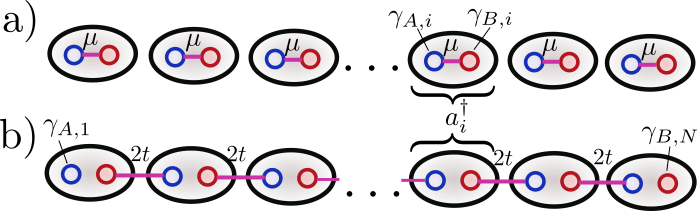
\includegraphics[scale=0.5]{IMAGES/Majorana/KitaevChain.png}
    \label{fig:top.phases kitaev}
    \caption{Illustration of the Kitaev chain for open boundary conditions in the Majorana representation. a)Represents the trivial case where the hopping and the superconducting term approaches to $0$. b) The non-trivial topological phase. The coupling is produced between Majoranas in different Dirac fermions \protect\Source{By the author} }
\end{figure}



The non-trivial phase An explanation to this phase transition can be given in terms of the topological 





% -----------------------Section: Modern and Experimental-------------
\section{Real implementations of majorana chains}


% -----------------------Leaking majorana modes in quantum dots-------------
\section{Leaking of Majorana modes in QDs}


